\section{Extreme value theory}
\label{sec:evt}
\subsection{Background}
By its nature the mean SSH will
not be able to damage the coast
(barring significant sea level rise that is not mitigated),
and life and property will only be put
at risk by the most extreme events~\cite{taleb2019statistical}.
Extreme value theory is the provides the necessary tools for this analysis
to look at the return period of extreme events of a certain value.
The two primary EVT methods are Peak over Threshold (POT) and Block Maxima (BM).
Both of these strategies require
large amounts of data to converge~\cite{taleb2019much} (e.g.~\texttt{c50}).
BM leads to Generalised Extreme Value (GEV) distribution,
whereas POT\footnote{Y20~\cite{ZannaPreprint} used POT methods. }
leads to Generalised Pareto Distribution (GPD).
Both require domain of attraction condition~\cite{bucher2018horse}, which
for BM is
$\forall r \in \mathbb{N} \;\exists \;b_r, \gamma\in \mathbb{R},\; a_r>0: $
    \begin{align}
    \lim _{r \rightarrow \infty} F^{r}\left(a_{r} x+b_{r}\right)=\exp \left\{-(1+\gamma x)^{-1 / \gamma}\right\} \notag \\
     \text { for all } 1+\gamma x>0,
    \tag{BM-DAC}
    \end{align}

which if fulfilled leads to:


    \(
    \operatorname{GEV}(\mu, \sigma, \xi):
    \)

    \(
    \text{ location, position of the GEV mean } \mu \in \mathbb{R};
    \)

    \(
    \text{scale, } \sigma>0;
    \)

    \(
    \text{shape, } \xi \in \mathbb{R}.
    \)

    \begin{align}
    \operatorname{GEV}(x; \mu, \sigma, \xi)=&
    \frac{1}{\sigma} \chi(x)^{1-\xi} e^{-\chi(x)}; \tag{GEV-1}
    \label{eq:GEV-1}
    \end{align}
    \begin{align}
    \chi(x)=&\left\{\begin{array}{ll}
    \left(1-\xi\left(\frac{x-\mu}{\sigma}\right)\right)^{1 / \xi} & \text { if } \xi \neq 0 \\
    e^{-(x-\mu) / \sigma} & \text { if } \xi=0 \tag{GEV-2}
    \end{array}\right.
    \label{eq:GEV-2}

    \end{align}


    A GEV with $\xi>0$, $\xi=0$, $\xi<0$ are
    respectively called the Weibull, Gumbel, and Fr\'echet
    distributions.\footnote{Here I have used the opposite sign convention for
    the shape, $\xi$, than is more commonly used. Please check against the
    forms of \ref{eq:GEV-1}~\&~\ref{eq:GEV-2} before interpreting results. }

\subsection{Block maxima GEV}
The highest SSH value in a given year at a given point
is extracted from \texttt{control-1950}, yielding 101 values per point.
It was decided not to subtract the seasonal SSH cycle from these
values, as it is the absolute height of the sea surface which
creates the hazard rather than the relative height.

\begin{figure*}[htb!]
    \centering
    \includegraphics[width=0.8\linewidth]{../surge/plots/GEV_modelNO.pdf}
    %\vspace{-25pt}
   \caption{New Orleans GEV plot for \texttt{control-1950} Interesting transition
            - does this represent hurricanes?}
    \label{fig:gev-no}
    \includegraphics[width=0.8\linewidth]{../surge/plots/skextreme_second_tactic.pdf}
    \vspace{-15pt}
   \caption{Confidence intervals not defined near Miami and Eastport. }
    \label{fig:gev_all_points}
\end{figure*}


\begin{figure*}[htb!]

\begin{minipage}{0.45\textwidth}

\includegraphics[width=1\linewidth]{../surge/plots/GEV_pi_plateau_NO.pdf}
\caption{First attempt at enforcing a GP asymptote of 2m for New Orleans,
with an \texttt{RBF} kernel.
The data is the same as in Figure~\ref{fig:gev-no}. The
kink is caused by using a non-differentiable mapping to
enforce the far-field conditions. 1$\sigma$ and 2$\sigma$ envelopes shown.}
\end{minipage}
\begin{minipage}{0.45\textwidth}

    \centering
    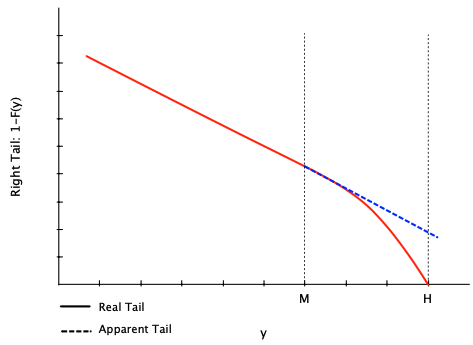
\includegraphics[width=1\linewidth]{images/taleb-limit-slimmed.png}\\
    \textit{Figure 15.1 from T19~\cite{taleb2019statistical} p.~279}
   \caption{As shown if you only
   observe a distribution up to some value M,
    you may be tempted to fit a line through the
   data (dotted blue line).
   But if there were in fact a limit to the distribution at H,
   you would be overestimating
   the true number of very extreme events (red curve),
   predicting events that were larger than were possible.}
   \label{fig:up-bound-taleb}
   \end{minipage}

   \begin{minipage}{0.45\textwidth}
   \centering
   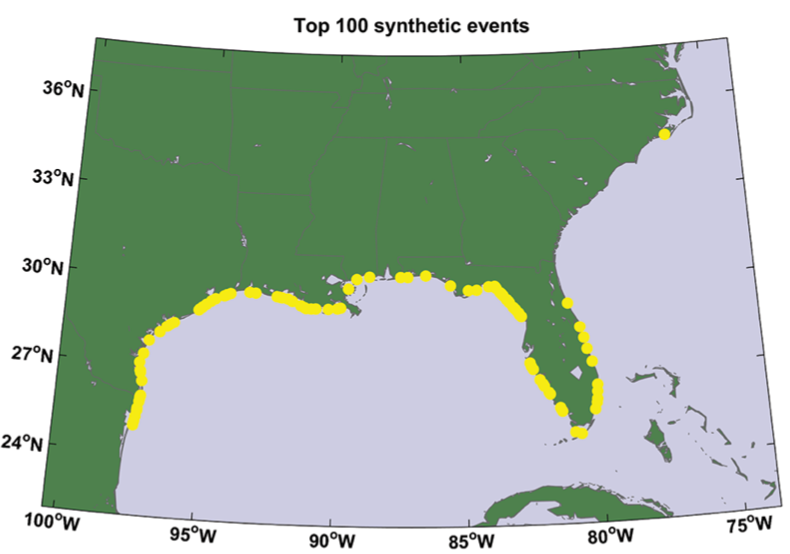
\includegraphics[width=1\linewidth]{images/top-100-landfalls.png}\\
   \textit{Figure 3b from \cite{emanuel2017will}}
   \caption{The top 100 most rapidly intensifying events in the model,
   showing that models capture far more of these TCs in the Gulf of Mexico
   and Florida than further north.
     }
   \label{fig:top-100}
   \end{minipage}
   \begin{minipage}{0.45\textwidth}
   \centering
   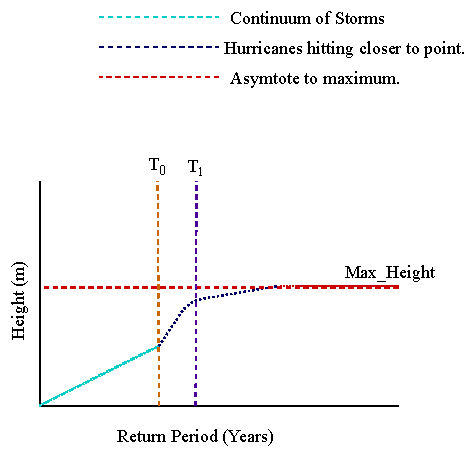
\includegraphics[width=1\linewidth]{images/Return_Hypothesis.pdf}
   \vspace{-15pt}
  \caption{The maximum height is a function of the potential intensity
  allowed by the climate, and the responsiveness of that point on the coastline to a
  wind stress of that size. If T$_0$, or T$_1$, is a similar or greater than the time period of
  measurement, then it is respectively possible that no hurricanes exist in the data sample,
  or that no hurricanes make direct landfall at that location.}
    \label{fig:return_hyp_new}
    \end{minipage}





\end{figure*}





Using my adaptation of \texttt{skextremes}~\cite{skextremes} I fit the
GEV with an initial guess from \texttt{lmoments}, optimised using
\texttt{scipy.stats.genextreme} with \texttt{scipy.optimize.fmin\_bfgs}~\cite{2020SciPy-NMeth}.
For some confidence interval, $\alpha$, the symmetric range of the parameters is
estimated by the delta method~\cite{coles2001introduction},

\begin{equation}
[\Delta \sigma , \Delta \mu, \Delta \xi] =
\mathcal{N}^{-1}(0, [\sigma_e (\sigma), \sigma_e (\mu), \sigma_e (\xi)]; 1-\frac{\alpha}{2})
\end{equation}

where,

\begin{equation}
[\sigma_e (\sigma), \sigma_e (\mu), \sigma_e (\xi)] =
\mathrm{sqrt}\left(\mathrm{diag}\left(\left( \mathrm{Hess}([\sigma, \mu, \xi]) \right)^{-1} \right)\right).
\end{equation}

We then also work out the uncertainty in each point in the
return plot fits (Figure~\ref{fig:gev-no}~C).

\begin{align}
\delta \mathbf{Z} = & \left[ \begin{array}{l}(\sigma\cdot\xi^{-2} \cdot (1-(\mathrm{sT}^{-\xi})
            \\-\sigma \cdot (\xi^{-1})\cdot (\mathrm{sT}^{-\xi}) \cdot \log(\mathrm{sT}[i])),\\
            1,\\
            -(1- \frac{\mathrm{sT}^{-\xi}}{\xi})
            \end{array} \right]
\end{align}

\begin{equation}
\sigma_e(\mathrm{sT2})^{2} = \mathrm{sqrt}\left((\delta \mathbf{Z} \cdot \left( \mathrm{Hess}([\sigma, \mu, \xi]) \right)^{-1} ) \cdot  \delta \mathbf{Z}^{\mathrm{T}}\right)
\end{equation}

Figure~\ref{fig:gev-no} fits the generalised extreme value theorem fitted
on the yearly block maxima for the nearest coastal point to New Orleans,
and Figure~\ref{fig:gev_all_points} shows the fit along all points in \texttt{eUS}
for \texttt{c50}.

\subsection{Enforcing an asymptote using potential intensity theory }
\label{sec:evt-limit}

As noted in~§~\ref{sec:hurr-theory} there is some maximum size
that a tropical cyclone might be expected to be able to reach given
the climate.
As shown in Figure~\ref{fig:up-bound-taleb} naively fitting
the GEV to the distribution would be an over-extrapolation of
the relationship if we have a good physical reason for
thinking that there is a maximum
(i.e.~the PI theory §~\ref{sec:hurr-theory}).

A hypothesis to explain the observed pattern of return periods is explained in
Figure~\ref{fig:return_hyp_new}, where the PI of hurricanes is used to
explain the flattening of the extreme
value with return period (see Figure~\ref{fig:eman-pi}).
However, absence of evidence is not
 evidence of absence, and some areas of the US
coastline such as Galverston and New England experience hurricanes infrequently
(due to cyclogenesis as in Figure~\ref{fig:genesis}),
but as respectively in 1900 and 1938,
when they do come they can cause great devastation~\cite{emanuel2005divine}.
The low TC frequency bias in CMIP models will exacerbate this problem.
This will appear as the blue curve continued without reaching the true plateau.
The period of time between T$_0$ and T$_1$ likely depends
 on the average size of the tropical cyclone storms,
and the percentage of them which rise to their maximum severity.
For highly irresponsive places (e.g.~Miami),
 it is possible that the deviation caused
by hurricane landfall does not cause a large
deviation from the existing EV distribution,
that is mainly caused by other factors (the Florida current).

A test for this hypothesis would be to use longer control runs from the same
coastline and model, to check that the deviation is not merely a problem caused
by chance, due to the length of time that BM takes to converge to GEV.

\begin{table}[h!]
    \centering
    \begin{tabular}{ll}
    \hline \hline
    \textbf{Sym} & \textbf{Description} \\
    \hline
        $\sigma$ & Scale. \\
        $\xi$ & Shape. \\
        $\mu$ & Location. \\
        $\sigma_e(.)$ & The standard devation of a parameter (.)\\
        Hess & The Hessian.\\
        diag & The diagonalization of the matrix. \\
        sqrt & Element wise square root.\\
        \alpha & The significance level (at 0.05 in Figure~\ref{fig:gev-no}.)\\
        $\delta \mathbf{Z}$&  \\
        sT & \\
        sT2 & \\
    \hline \hline
    \end{tabular}
    \caption{Symbols (Sym) for extreme value theory.}
    \label{tab:fluid_variables}
\end{table}


\begin{figure}[htb!]
    \centering
    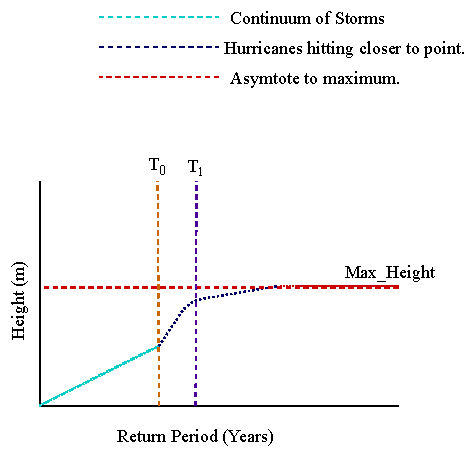
\includegraphics[width=1\linewidth]{images/Return_Hypothesis.pdf}
    \vspace{-15pt}
   \caption{The maximum height is a function of the potential intensity
   allowed by the climate, and the responsiveness of that point on the coastline to a
   wind stress of that size. If T$_0$, or T$_1$, is a similar or greater than the time period of
   measurement, then it is respectively possible that no hurricanes exist in the data sample,
   or that no hurricanes make direct landfall at that location.}
     \label{fig:return_hyp_new}

\end{figure}


\begin{figure*}
\centering
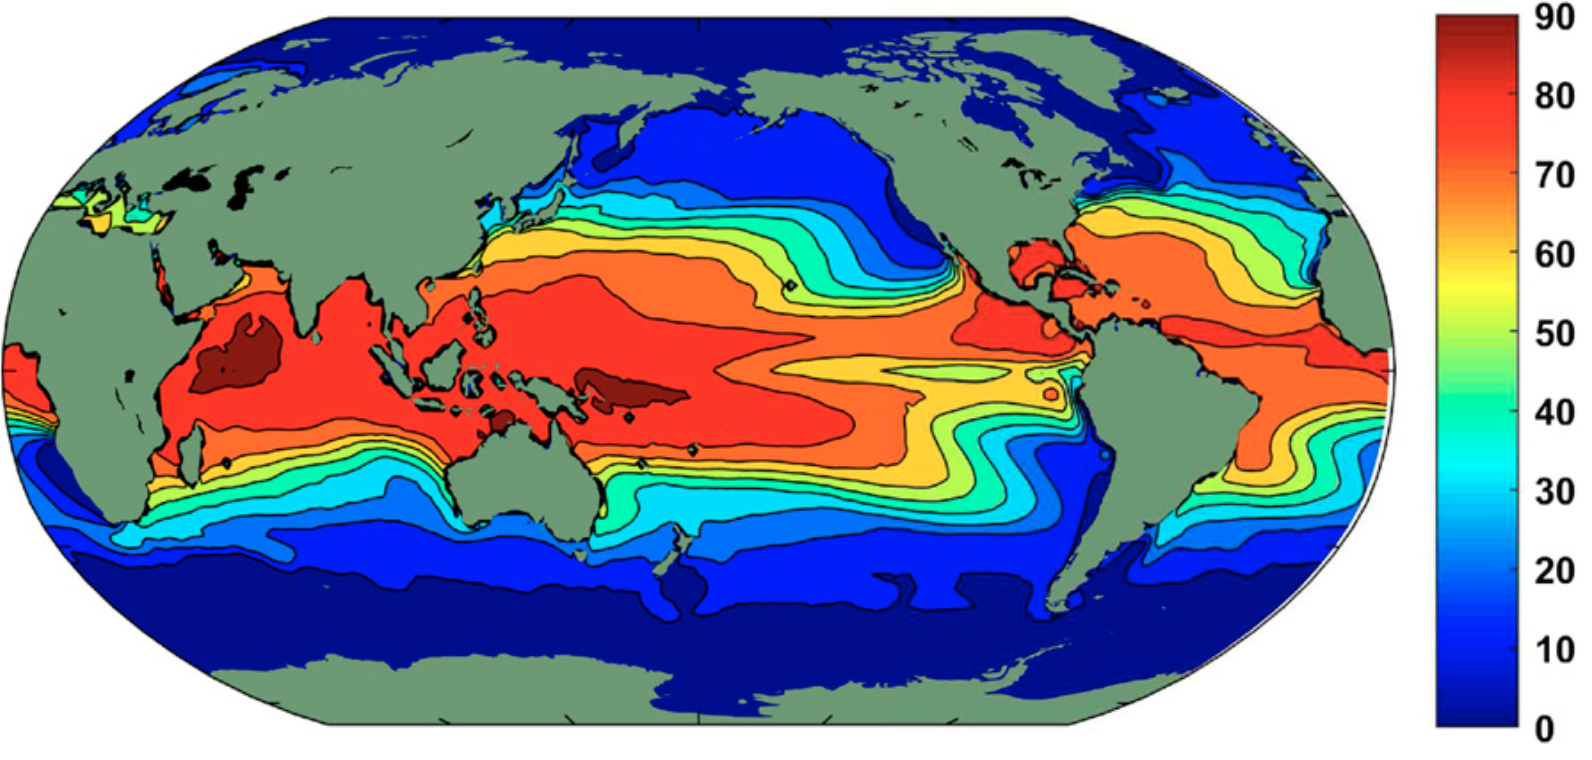
\includegraphics[width=\linewidth]{images/PI-max-year.png}\\
\textit{Figure 15-7 from \cite{emanuel2018progress}.}
\caption{The annual maximum of the potential intensity (m s$^{-1}$), calculated using
~\cite{bister2002low} and ERA-Interim data 1979-2016.
This is product maps on well to the block maxima procedure in §~\ref{sec:evt}.
}
\label{fig:eman}
\end{figure*}




\FloatBarrier
